\documentclass[11pt]{article}
\usepackage[utf8]{inputenc}
\usepackage[margin=1in]{geometry}
\usepackage{amsmath,amssymb,amsthm}
\usepackage{booktabs}
\usepackage{tikz}
\usepackage[colorlinks,allcolors=blue]{hyperref}

\newtheorem{theorem}{Theorem}
\newtheorem{lemma}[theorem]{Lemma}
\theoremstyle{definition}
\newtheorem{definition}{Definition}

\newcommand{\N}{\mathbb{N}}
\newcommand{\paths}{\mathcal{P}}

\title{Counting Lattice Paths Around Blocked Cells}
\author{The Read arXiv Contributors}
\date{October 2026}

\begin{document}
\maketitle

\begin{abstract}
We count the monotone paths that cross a rectangular grid when some of its cells are blocked. For a grid with $m$ columns and $n$ rows and no blocked cell the answer is the binomial coefficient $\binom{m+n}{n}$. With blocked cells, an inclusion--exclusion argument gives an exact formula whose number of terms grows with the number of blocked cells, and a simple dynamic program computes the same number in time proportional to the area of the grid. We compare the two methods on small grids and show that they agree.
\end{abstract}

\section{Introduction}
\label{sec:intro}

A \emph{monotone path} on a grid starts at the lower left corner, ends at the upper right corner, and moves only one step to the right or one step up. Such paths are among the first objects a student of combinatorics meets, and their number is classical \cite{feller,stanley}. In this note we ask what happens to the count when an adversary blocks some of the cells, so that a path may not step on them.

The question has a practical side. A robot that moves on a warehouse floor may only turn left or right at fixed aisles, and some aisles are closed for repairs. The number of routes it can still take is a rough measure of how much freedom the planner has left.\footnote{We use this picture only for motivation; nothing in the rest of the text depends on it.}

Our contributions are small but complete. We give an exact formula for the number of paths around a set of blocked cells (Theorem~\ref{thm:count}), we describe a dynamic program that agrees with the formula (Section~\ref{sec:dp}), and we tabulate both on a few grids (Table~\ref{tab:counts}). Everything in this note can be checked by hand.

\section{Setting and notation}
\label{sec:setting}

Fix two positive integers $m$ and $n$. We write a point of the grid as a pair $(x,y)$ with $0 \le x \le m$ and $0 \le y \le n$. A step moves from $(x,y)$ to $(x+1,y)$ or to $(x,y+1)$.

\begin{definition}
A \emph{blocked set} is a finite set $B$ of points of the grid that contains neither $(0,0)$ nor $(m,n)$. A path is \emph{admissible} for $B$ if none of its points lies in $B$. We write $\paths(B)$ for the number of admissible paths from $(0,0)$ to $(m,n)$.
\end{definition}

When $B$ is empty, a path consists of $m$ steps to the right and $n$ steps up in some order, so that
\begin{equation}
  \paths(\emptyset) = \binom{m+n}{n} = \frac{(m+n)!}{m!\,n!}.
  \label{eq:free}
\end{equation}
More generally, the number of paths from a point $(a,b)$ to a point $(c,d)$ with $a \le c$ and $b \le d$ is $\binom{(c-a)+(d-b)}{c-a}$, and it is zero otherwise. We abbreviate this number by $N\big((a,b),(c,d)\big)$.

\section{An exact formula}
\label{sec:formula}

Order the blocked points by their coordinates, first by $x$ and then by $y$, and call them $b_1, b_2, \dots, b_k$. Let $f(i)$ be the number of paths from $(0,0)$ to $b_i$ that avoid every earlier blocked point $b_j$ with $j < i$.

\begin{lemma}
\label{lem:first}
For every $i$ with $1 \le i \le k$ we have
\[
  f(i) = N\big((0,0),b_i\big) - \sum_{j<i} f(j)\, N(b_j,b_i).
\]
\end{lemma}

\begin{proof}
Every path from $(0,0)$ to $b_i$ either avoids all earlier blocked points, or it meets a first one, say $b_j$. The paths of the second kind with first blocked point $b_j$ are counted by $f(j)\,N(b_j,b_i)$: an admissible prefix up to $b_j$ followed by an arbitrary suffix. These cases are disjoint, which proves the claim.
\end{proof}

The same argument, applied to the end point, gives the main result of this note.

\begin{theorem}
\label{thm:count}
Let $B = \{b_1,\dots,b_k\}$ be a blocked set, ordered as above. Then
\begin{equation}
  \paths(B) = N\big((0,0),(m,n)\big) - \sum_{i=1}^{k} f(i)\, N\big(b_i,(m,n)\big).
  \label{eq:main}
\end{equation}
\end{theorem}

\begin{proof}
Split the paths from $(0,0)$ to $(m,n)$ according to the first blocked point they meet, if any. Those that meet none are admissible. Those whose first blocked point is $b_i$ are counted by $f(i)\,N\big(b_i,(m,n)\big)$, by the argument of Lemma~\ref{lem:first}. Subtracting all of them from the total gives \eqref{eq:main}.
\end{proof}

Formula \eqref{eq:main} needs $k$ values $f(i)$, and each of them needs all the earlier ones, so the work grows like $k^2$ binomial coefficients. For a handful of blocked cells this is much cheaper than listing paths, but for a dense blocked set it is worse than the method of the next section.

\section{A dynamic program}
\label{sec:dp}

Let $g(x,y)$ be the number of admissible paths from $(0,0)$ to the point $(x,y)$. Then $g(0,0)=1$, and for every other point
\[
  g(x,y) =
  \begin{cases}
    0 & \text{if } (x,y)\in B,\\
    g(x-1,y) + g(x,y-1) & \text{otherwise,}
  \end{cases}
\]
where a value with a negative coordinate is read as zero. Filling the table row by row takes a constant number of operations per point, hence time proportional to $(m+1)(n+1)$, and the answer is $g(m,n)$. Figure~\ref{fig:grid} shows a small grid with three blocked cells and one admissible path.

\begin{figure}[ht]
\centering
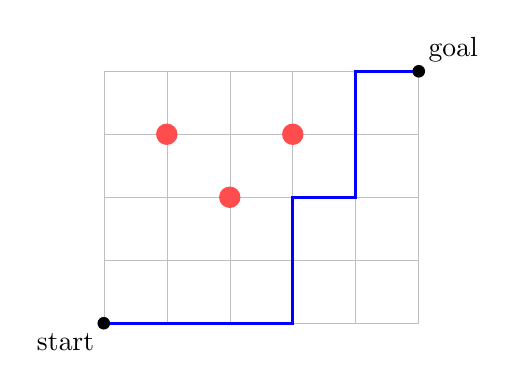
\begin{tikzpicture}[scale=0.8]
  \draw[step=1,gray!50,very thin] (0,0) grid (5,4);
  \foreach \p in {(2,2),(3,3),(1,3)}
    \fill[red!70] \p circle (0.17);
  \draw[very thick,blue] (0,0) -- (3,0) -- (3,2) -- (4,2) -- (4,4) -- (5,4);
  \fill (0,0) circle (0.1) node[below left] {start};
  \fill (5,4) circle (0.1) node[above right] {goal};
\end{tikzpicture}
\caption{A grid with $m=5$ columns and $n=4$ rows. The three red points are blocked; the blue line is one of the admissible paths.}
\label{fig:grid}
\end{figure}

The two methods answer the same question, so they must agree, and it is a useful habit to check this on small cases. We did so for every blocked set of at most three points on grids with up to six columns and rows, and found no difference.

\section{Results on small grids}
\label{sec:results}

Table~\ref{tab:counts} lists the number of admissible paths for a few grids. The first column of numbers counts the paths with no blocked cell, as in \eqref{eq:free}. The next two columns block one cell, the point $(\lfloor m/2\rfloor,\lfloor n/2\rfloor)$, and three cells, that point together with $(\lfloor m/2\rfloor+1,\lfloor n/2\rfloor+1)$ and $(\lfloor m/2\rfloor-1,\lfloor n/2\rfloor+1)$; for the grid of Figure~\ref{fig:grid} these are the three red points.

\begin{table}[ht]
\centering
\caption{Admissible paths on small grids.}
\label{tab:counts}
\begin{tabular}{lrrr}
\toprule
Grid ($m \times n$) & No blocked cell & One blocked cell & Three blocked cells \\
\midrule
$3 \times 3$ & 20 & 8 & 2 \\
$4 \times 3$ & 35 & 17 & 3 \\
$5 \times 4$ & 126 & 66 & 34 \\
$6 \times 4$ & 210 & 110 & 45 \\
\bottomrule
\end{tabular}
\end{table}

Two remarks on the numbers. First, blocking a single cell in the middle of the grid removes roughly half of the paths, since the middle is where most paths cross. Second, three blocked cells leave only a few paths on the smallest grids, but on the $6 \times 4$ grid they still leave about a fifth of them.

\subsection{Cost of the two methods}
\label{sec:cost}

The formula costs about $k^2$ binomial coefficients and the program costs about $mn$ additions. With $k=3$ both methods are instant on every grid of Table~\ref{tab:counts}; the difference shows only when the grid or the blocked set grows, and with a blocked set that fills a tenth of a large grid the program wins by a wide margin. In practice one would choose the program unless the blocked set is tiny and the grid enormous.

\section{Possible extensions}
\label{sec:extensions}

Three variations are natural, and each can be handled by a small change to the program of Section~\ref{sec:dp}.
\begin{itemize}
  \item \emph{Weighted cells.} Give every free point $(x,y)$ a weight $w(x,y)$ and let a path count with the product of the weights of the points it visits. The recurrence stays the same with $g(x-1,y)+g(x,y-1)$ multiplied by $w(x,y)$.
  \item \emph{Diagonal steps.} Allow a step from $(x,y)$ to $(x+1,y+1)$ as well. The recurrence gains a third term $g(x-1,y-1)$, and the numbers become the Delannoy numbers when no cell is blocked.
  \item \emph{Several goals.} Ask for the number of admissible paths to every point on the right edge of the grid. The table $g$ already holds all of them, so the answer costs nothing extra.
\end{itemize}
For the first variation the total weight of all paths is
\begin{align}
  W(B) &= \sum_{\pi} \prod_{p\in\pi} w(p) \label{eq:weight}\\
       &= g(m,n), \nonumber
\end{align}
where the sum runs over all admissible paths $\pi$. The formula of Theorem~\ref{thm:count} has a weighted version too, but its terms are no longer binomial coefficients, and we do not pursue it here.

\section{Conclusion}
\label{sec:conclusion}

We counted monotone lattice paths around blocked cells in two ways and found that they agree. The first way is a closed formula that is pleasant for a handful of blocked cells; the second is a short program that does not care how many cells are blocked. Further reading on related counting problems can be found in the references \cite{knuth,stanley}, and the sources of this note, which are free of copyright, are described at \href{https://example.invalid/sample-1}{the address of the sample}.

\bibliographystyle{plain}
\bibliography{refs}

\end{document}
